\clearpage
\section{Kardinalistické pojetí chování spotřebitele (princip, definice mezního a celkového
užitku, rovnováha spotřebitele při spotřebě jednoho statku, přebytek spotřebitele,
rovnováha spotřebitele při spotřebě dvou a více statků) a odvození individuální
poptávky.}

\subsection{Princip}
\begin{itemize}
    \item Spotřebitel dokáže vyjádřit užitek v peněžních jednotkách
    \item Nakupuje, dokud se mezní užitek nerovná ceně statku
\end{itemize}

\subsection{Mezní užitek}
Přírůstek užitku s každou další pořízenou jednotkou statku, klesá s množstvím pořízených statků.

\subsection{Celkový užitek}
Součet všech mezních užitků, užitek ze všech pořízených statků. S každou další jednotkou roste,
ale \textit{rychlost přírůstku} se snižuje s každou další jednotkou (konkávní funkce).

\subsection{Rovnováha spotřebitele při spotřebě jednoho statku}
Nastává, pokud se tržní cena statku rovná meznímu užitku z nákupu tohoto statku.

\subsection{přebytek spotřebitele}
Jedná se o rozdíl celkové ceny, kterou byl zákazník ochotný zaplatit a ceny, za které byly opravdu statky nakoupeny. \\
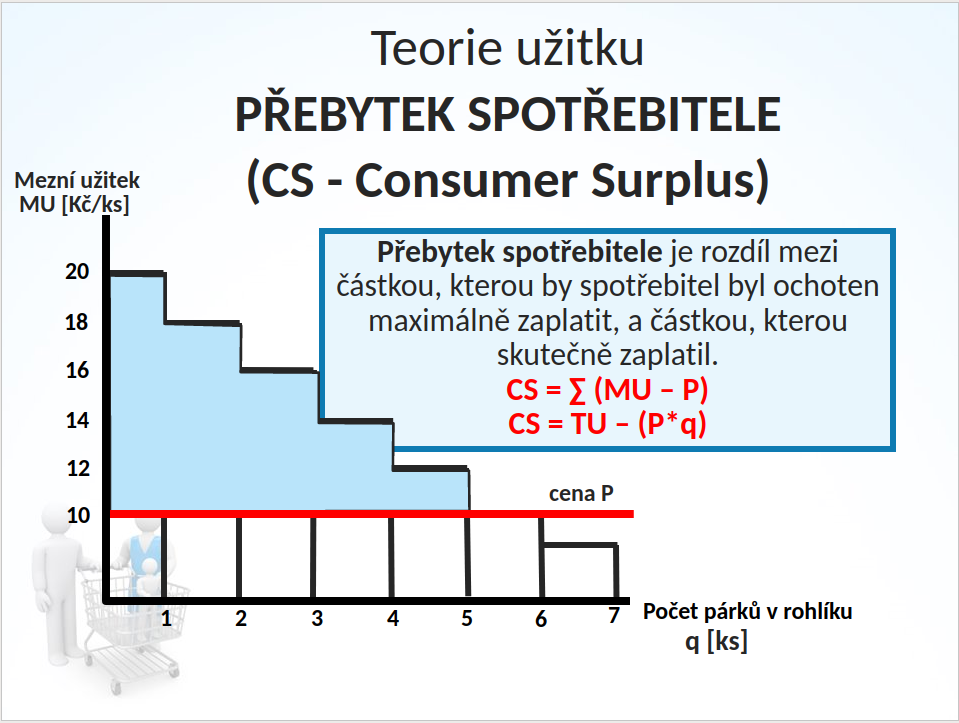
\includegraphics[width=16cm]{images/prebytek_spotrebitele.png}

\subsection{Rovnováha spotřebitele při spotřebě dvou a více statků}
Musí platit, že poměr mezních užitků a cen jednotlivých statků je stejný pro všechny statky. \\
$\frac{MU_1}{P_1}=\frac{MU_2}{P_2}=\dots=\frac{MU_n}{P_n}$

\subsection{Odvození individuální poptávky}
V tomto pojetí je chápána jednoduše jako funkce mezního užitku (klesající), jen nemůže jít do záporných hodnot. (Končí mezním užitkem rovným nule.)
